\documentclass[letterpaper]{article} % Feel free to change this

\usepackage{graphicx}
\usepackage[english]{babel}
\usepackage[utf8]{inputenc}
\usepackage{fancyhdr}
 
\pagestyle{fancy}
\fancyhf{}
\rhead{Week of Feb 4}
\lhead{CS 270 Helper Material}

\setlength\parindent{0pt}

\begin{document}

\section{Game Playing}

Most of the games we will study have the following properties:

\begin{enumerate}
	\item have two players
	\item are \textit{zero-sum}: what one player wins, the other loses
	\item have \textit{perfect information}: the entire state of the game is known to both players at all times
\end{enumerate}

An example of a game with \textit{imperfect information} is poker, where one player does not know the cards that the other player holds.

\subsection{Game Tree}

A game tree is used to display the potential outcomes of games. Nodes represent states, successors represent moves, and terminal nodes are assigned values based on who won/lost/tied. Below is an example of such a game tree.

\begin{figure}[h]
\centering
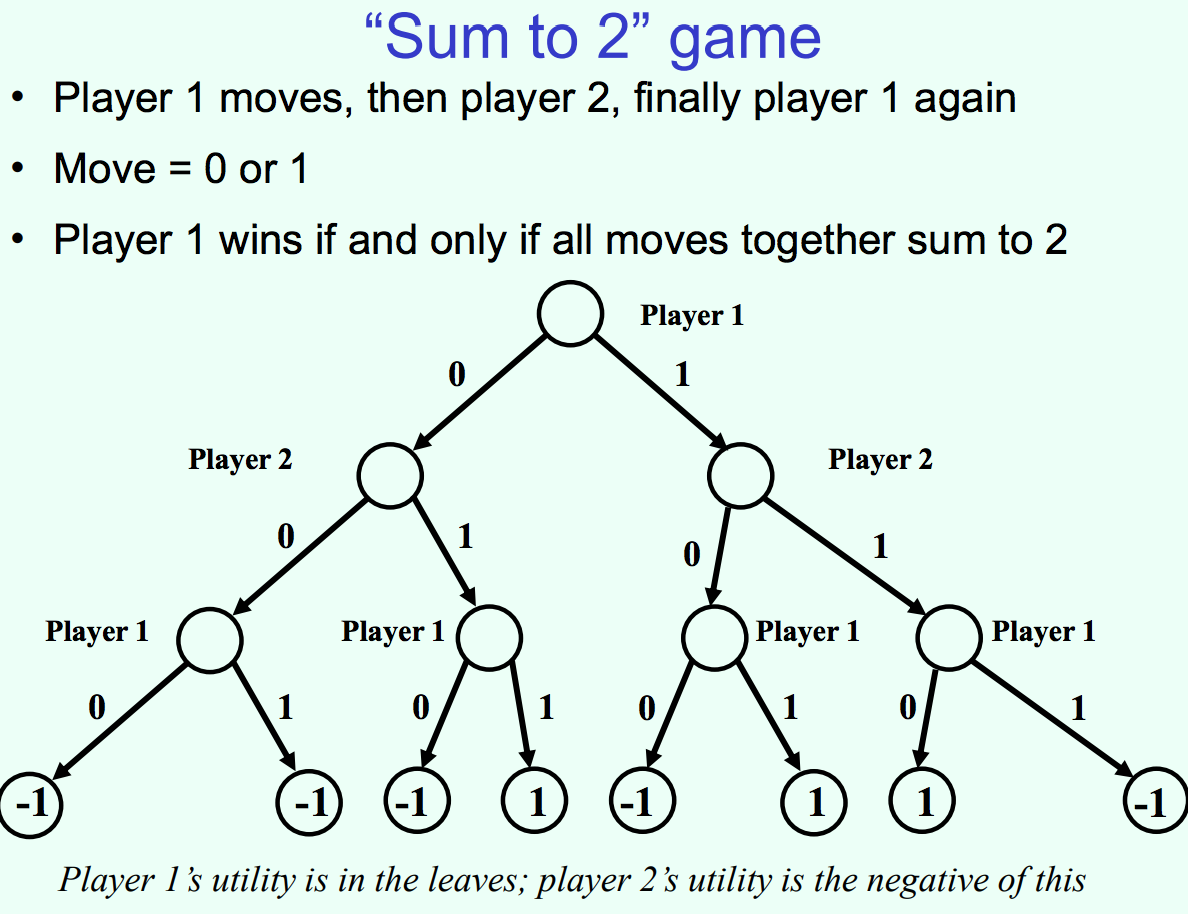
\includegraphics[width=8cm]{search_tree}
\caption{Example Search Tree}
\end{figure}

For the full game playing example, please see slides.

\subsection{Minimax}

Assume that a positive utility final state implies Player 1 wins, and Player 2 loses, and a negative utility final state implies Player 1 loses, and Player 2 wins. When given the choice over successors, Player 1 will always pick the successor that guarantees the maximum utility. Conversely, Player 2 will always select the successor that guarantees the minimum utility. These calls can be made recursively by cycling between maximizing the result which was minimized based on the results that were maximized and so on. Please see \textbf{Game Playing Slides (p6)} for the pseudo code of a basic implementation.\\

The implementation follows a depth first traversal. Therefore the space and time are equal to that of DFS. If you consider each move to be one person moves, and terminal nodes exist at a depth of $d$, and each player has $b$ possible moves they can make at any given turn, then:\\

Space: $bd$

Time: $b^d$

\subsection{Alpha Beta Pruning}

Maintains the best option for Player 1 ($\alpha$), and Player 2 ($beta$). Using this information players are able to skip over branches of the game tree. The extent to which branches are pruned depends on the order which branches are explored. More specifically, branches where $alpha \ge \beta$ can be pruned. Please see slides \textbf{Game Playing Slides p 12} for the pseudo code and to walk through a couple game trees. Students should be familiar doing alpha beta pruning on game trees in person using pencil and paper.

\subsubsection{Benefits Of Alpha Beta}

Without pruning, we need to evaluate $O(b^d)$ states. With random pruning, we need to examine $O(b^{\frac{3}{4}d})$, and if you are able to perfectly choose which branch to look at first, the number of states evaluated is $O(b^{\frac{1}{2}d})$. Under such a condition (perfect branch ordering), we can search to double the depth. This can make a significance difference in the game play achieved.

\subsection{What if searching to the end of the game is unfeasible?}

Under such a condition, it is not immediately obvious how to assign values to states (we don't know who will win!). In these cases, we use an evaluation function. An evaluation function, assigns a score to a state, which is intended to estimate the cost if both agents played optimally from that state onward. For example, each piece in chess is worth a certain amount of points.\\

Let's say a node is \textbf{quiescent} if the evaluation function will not change rapidly in the near future. Can be thought of as a measure of stability. Choosing successors that lead to quiescent states can protect against stepping into a highly volatile state.

\subsection{Games of Nature}

Games of nature are the subset of games where a player makes a choice based on random chance. For example, given two successors $A$ and $B$, a nature player will pick successor $A$ with probability $P_A$ and will pick $B$ with probability $P_B$ such that $P_A + P_B = 1$. Rather than minimaxing the value of these choices, we take the weighted average of the successor where the weights are equal to the probability of each choice. 

\section{Propositional Logic}

\subsection{Syntax}

A Backus–Naur Form, or Backus Normal Form, (BNF) grammar takes the following form\\

$Symbol => P, Q, R, isRaining, etc$\\

$Sentence => True$

$\quad\quad\quad\quad\quad | \quad False$

$\quad\quad\quad\quad\quad | \quad Symbol$

$\quad\quad\quad\quad\quad | \quad NOT(Sentence)$

$\quad\quad\quad\quad\quad | \quad (Sentence \quad AND \quad Sentence)$

$\quad\quad\quad\quad\quad | \quad (Sentence \quad OR \quad Sentence)$

$\quad\quad\quad\quad\quad | \quad (Sentence => Sentence)$

\subsection{Semantics}

A \textbf{model} specifies which of the proposition symbols are true and which are false.\\

Given a model you should be able to determine if a sentence is true or false. Truth tables can be used to define the semantics of every operator.\\

A sentence is a \textbf{tautology} if it is true for any setting of its propositional statements. For example $(\alpha \quad OR \quad True)$ will always evaluate to true, no matter what $\alpha$ is. Please see famous logical equivalences on slide 11 of the logic slides to see useful logical axioms and derived properties.

\end{document}
